% Options for packages loaded elsewhere
\PassOptionsToPackage{unicode}{hyperref}
\PassOptionsToPackage{hyphens}{url}
\PassOptionsToPackage{dvipsnames,svgnames,x11names}{xcolor}
%
\documentclass[
]{agujournal2019}

\usepackage{amsmath,amssymb}
\usepackage{iftex}
\ifPDFTeX
  \usepackage[T1]{fontenc}
  \usepackage[utf8]{inputenc}
  \usepackage{textcomp} % provide euro and other symbols
\else % if luatex or xetex
  \usepackage{unicode-math}
  \defaultfontfeatures{Scale=MatchLowercase}
  \defaultfontfeatures[\rmfamily]{Ligatures=TeX,Scale=1}
\fi
\usepackage{lmodern}
\ifPDFTeX\else  
    % xetex/luatex font selection
\fi
% Use upquote if available, for straight quotes in verbatim environments
\IfFileExists{upquote.sty}{\usepackage{upquote}}{}
\IfFileExists{microtype.sty}{% use microtype if available
  \usepackage[]{microtype}
  \UseMicrotypeSet[protrusion]{basicmath} % disable protrusion for tt fonts
}{}
\makeatletter
\@ifundefined{KOMAClassName}{% if non-KOMA class
  \IfFileExists{parskip.sty}{%
    \usepackage{parskip}
  }{% else
    \setlength{\parindent}{0pt}
    \setlength{\parskip}{6pt plus 2pt minus 1pt}}
}{% if KOMA class
  \KOMAoptions{parskip=half}}
\makeatother
\usepackage{xcolor}
\setlength{\emergencystretch}{3em} % prevent overfull lines
\setcounter{secnumdepth}{5}
% Make \paragraph and \subparagraph free-standing
\makeatletter
\ifx\paragraph\undefined\else
  \let\oldparagraph\paragraph
  \renewcommand{\paragraph}{
    \@ifstar
      \xxxParagraphStar
      \xxxParagraphNoStar
  }
  \newcommand{\xxxParagraphStar}[1]{\oldparagraph*{#1}\mbox{}}
  \newcommand{\xxxParagraphNoStar}[1]{\oldparagraph{#1}\mbox{}}
\fi
\ifx\subparagraph\undefined\else
  \let\oldsubparagraph\subparagraph
  \renewcommand{\subparagraph}{
    \@ifstar
      \xxxSubParagraphStar
      \xxxSubParagraphNoStar
  }
  \newcommand{\xxxSubParagraphStar}[1]{\oldsubparagraph*{#1}\mbox{}}
  \newcommand{\xxxSubParagraphNoStar}[1]{\oldsubparagraph{#1}\mbox{}}
\fi
\makeatother


\providecommand{\tightlist}{%
  \setlength{\itemsep}{0pt}\setlength{\parskip}{0pt}}\usepackage{longtable,booktabs,array}
\usepackage{calc} % for calculating minipage widths
% Correct order of tables after \paragraph or \subparagraph
\usepackage{etoolbox}
\makeatletter
\patchcmd\longtable{\par}{\if@noskipsec\mbox{}\fi\par}{}{}
\makeatother
% Allow footnotes in longtable head/foot
\IfFileExists{footnotehyper.sty}{\usepackage{footnotehyper}}{\usepackage{footnote}}
\makesavenoteenv{longtable}
\usepackage{graphicx}
\makeatletter
\newsavebox\pandoc@box
\newcommand*\pandocbounded[1]{% scales image to fit in text height/width
  \sbox\pandoc@box{#1}%
  \Gscale@div\@tempa{\textheight}{\dimexpr\ht\pandoc@box+\dp\pandoc@box\relax}%
  \Gscale@div\@tempb{\linewidth}{\wd\pandoc@box}%
  \ifdim\@tempb\p@<\@tempa\p@\let\@tempa\@tempb\fi% select the smaller of both
  \ifdim\@tempa\p@<\p@\scalebox{\@tempa}{\usebox\pandoc@box}%
  \else\usebox{\pandoc@box}%
  \fi%
}
% Set default figure placement to htbp
\def\fps@figure{htbp}
\makeatother

\usepackage{url} %this package should fix any errors with URLs in refs.
\usepackage{lineno}
\usepackage[inline]{trackchanges} %for better track changes. finalnew option will compile document with changes incorporated.
\usepackage{soul}
\linenumbers
\makeatletter
\@ifpackageloaded{caption}{}{\usepackage{caption}}
\AtBeginDocument{%
\ifdefined\contentsname
  \renewcommand*\contentsname{Table of contents}
\else
  \newcommand\contentsname{Table of contents}
\fi
\ifdefined\listfigurename
  \renewcommand*\listfigurename{List of Figures}
\else
  \newcommand\listfigurename{List of Figures}
\fi
\ifdefined\listtablename
  \renewcommand*\listtablename{List of Tables}
\else
  \newcommand\listtablename{List of Tables}
\fi
\ifdefined\figurename
  \renewcommand*\figurename{Figure}
\else
  \newcommand\figurename{Figure}
\fi
\ifdefined\tablename
  \renewcommand*\tablename{Table}
\else
  \newcommand\tablename{Table}
\fi
}
\@ifpackageloaded{float}{}{\usepackage{float}}
\floatstyle{ruled}
\@ifundefined{c@chapter}{\newfloat{codelisting}{h}{lop}}{\newfloat{codelisting}{h}{lop}[chapter]}
\floatname{codelisting}{Listing}
\newcommand*\listoflistings{\listof{codelisting}{List of Listings}}
\makeatother
\makeatletter
\makeatother
\makeatletter
\@ifpackageloaded{caption}{}{\usepackage{caption}}
\@ifpackageloaded{subcaption}{}{\usepackage{subcaption}}
\makeatother

\usepackage{bookmark}

\IfFileExists{xurl.sty}{\usepackage{xurl}}{} % add URL line breaks if available
\urlstyle{same} % disable monospaced font for URLs
\hypersetup{
  pdftitle={Яка машиночитаність потрібна для доступності використання відкритих даних},
  pdfauthor={Микола Кузін},
  pdfkeywords={машиночитаність, відкриті дані},
  colorlinks=true,
  linkcolor={blue},
  filecolor={Maroon},
  citecolor={Blue},
  urlcolor={Blue},
  pdfcreator={LaTeX via pandoc}}



\draftfalse

\begin{document}
\title{Яка машиночитаність потрібна для доступності використання
відкритих даних}

\authors{Микола Кузін\affil{1}}
\affiliation{1}{BRDO, }
\correspondingauthor{Микола Кузін}{m.kuzin@brdo.com.ua}


\begin{abstract}
Говорячи про машиночитаність, слід розрізняти
\end{abstract}





\section{Вільний доступ vs доступність використання відкритих
даних}\label{ux432ux456ux43bux44cux43dux438ux439-ux434ux43eux441ux442ux443ux43f-vs-ux434ux43eux441ux442ux443ux43fux43dux456ux441ux442ux44c-ux432ux438ux43aux43eux440ux438ux441ux442ux430ux43dux43dux44f-ux432ux456ux434ux43aux440ux438ux442ux438ux445-ux434ux430ux43dux438ux445}

За визначенням Open Knowledge Foundation, розробників CKAN, на якій
реалізований український Портал відкритих даних, ``відкритість'' даних
полягає в тому, що будь-хто може мати до них вільний доступ, вільно
використовувати, змінювати та ділитися ними.

Однак ``вільний'' не завжди значить ``відкритий'': часто потрібні
додаткові кроки, щоби з інформації у вільному доступі зробити дані,
доступні до використання.

У Постанові КМУ № 835 ``доступність використання'' відкритих даних
напряму пов'язується з машиночитаним форматом оприлюднених даних. А
машиночитаність --- зі структурованістю даних, що уможливлює обробку без
участі людини (власне, машинну обробку). У Постанові також визначено
перелік форматів (розширень) структурованих

Подивимося на значення машиночитаності в контексті відкритих даних і
поміркуємо

Free is not Always Open. Making data freely available is only the first
step in making it open for all to reuse. There are layers of barriers
between information that anyone can get and data that anyone can use.
This is because making the data open is not always about licences or the
format issues, but it is also about comprehension and access. Open data
should not require additional time, resources and expertise to be used.

``Open means~anyone~can~freely access, use, modify, and share~for~any
purpose~(subject, at most, to requirements that preserve provenance and
openness).''

Тому при відкритті даних слід зважати не лише на ліцензії та формати
даних, а й на сприйняття та доступність користувачеві.

Based on data up to and including 1971, eruptions on La Palma happen
every \texttt{\{r\}\ round(avg\_years\_between\_eruptions,\ 1)} years on
average.

Studies of the magma systems feeding the volcano, save proposed that
there are two main magma reservoirs feeding the Cumbre Vieja volcano;
one in the mantle (30-40km depth) which charges and in turn feeds a
shallower crustal reservoir (10-20km depth).

Eight eruptions have been recorded since the late 1400

Data and methods are discus

Let \(x\) denote the number of eruptions in a year. Then, \(x\) can be
modeled by a Poisson distribution

\begin{equation}\phantomsection\label{eq-poisson}{
p(x) = \frac{e^{-\lambda} \lambda^{x}}{x !}
}\end{equation}

where \(\lambda\) is the rate of eruptions per year. robability of an
eruption in the next \(t\) years can be calculated.

\begin{longtable}[]{@{}ll@{}}
\caption{Recent historic eruptions on La
Palma}\label{tbl-history}\tabularnewline
\toprule\noalign{}
Name & Year \\
\midrule\noalign{}
\endfirsthead
\toprule\noalign{}
Name & Year \\
\midrule\noalign{}
\endhead
\bottomrule\noalign{}
\endlastfoot
Current & 2021 \\
Teneguía & 1971 \\
Nambroque & 1949 \\
El Charco & 1712 \\
Volcán San Antonio & 1677 \\
Volcán San Martin & 1646 \\
Tajuya near El Paso & 1585 \\
Montaña Quemada & 1492 \\
\end{longtable}

the eruptions recorded since the colonization of the islands by
Europeans in the late 1400s.

\begin{figure}

\centering{

\pandocbounded{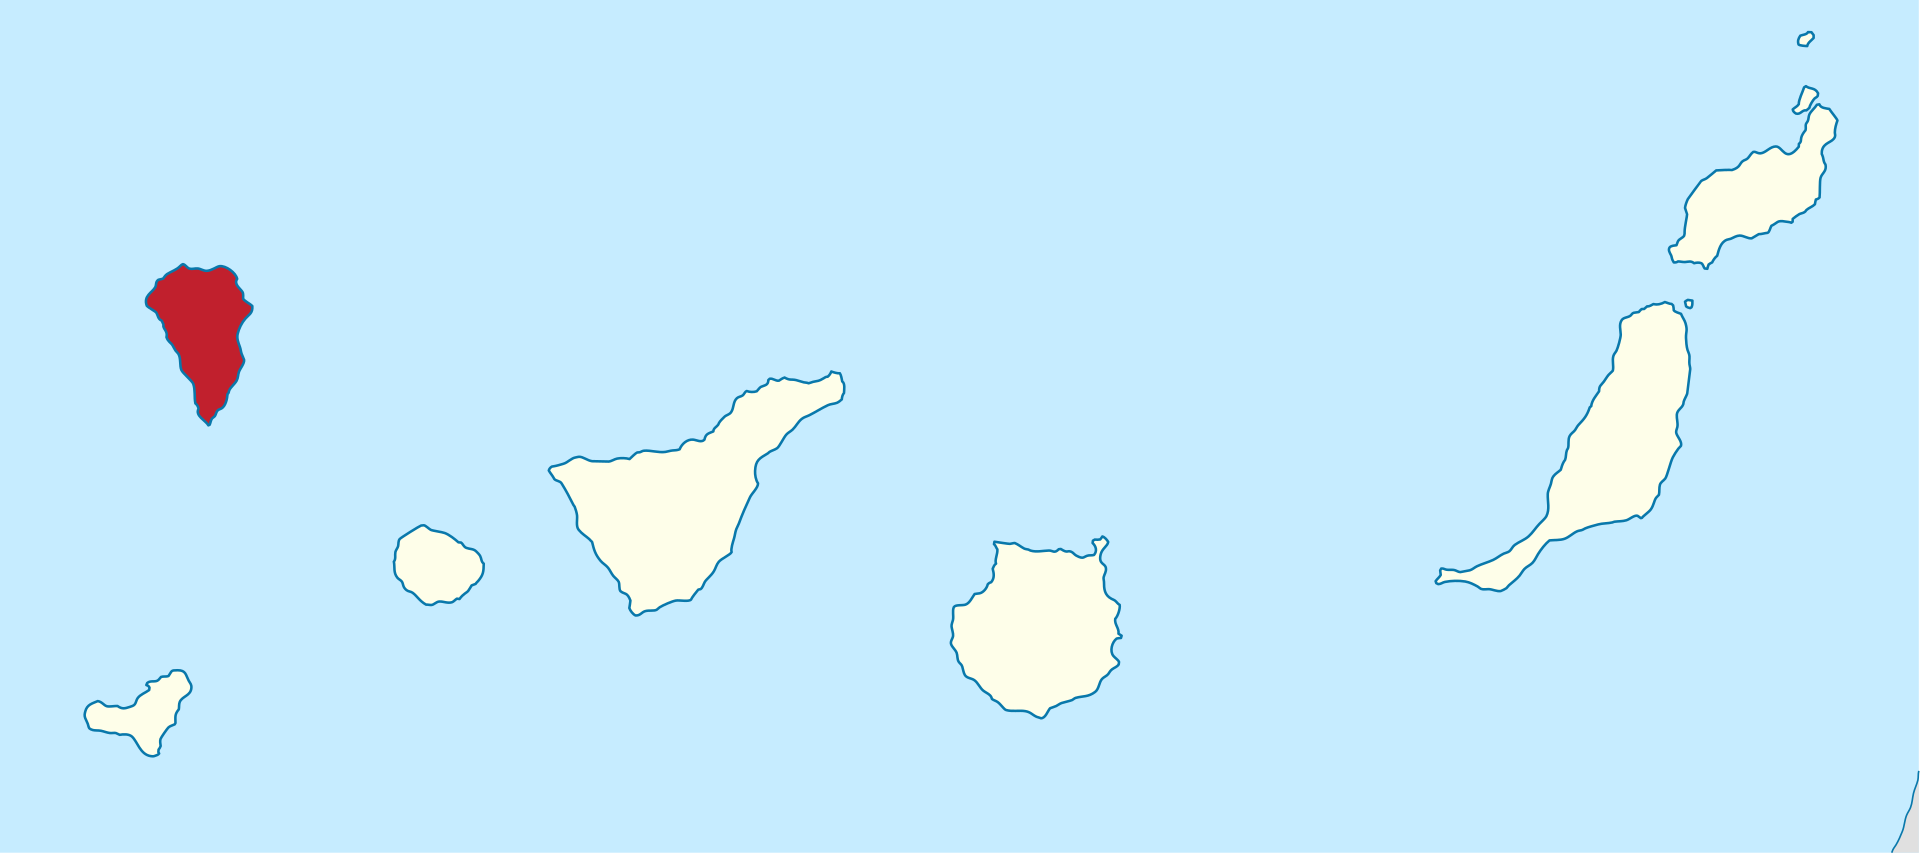
\includegraphics[keepaspectratio]{images/la-palma-map.png}}

}

\caption{\label{fig-map}Map of La Palma}

\end{figure}%

La Palma is one of the west most islands in the Volcanic Archipelago of
the Canary Islan

\section{Data \& Methods}\label{sec-data-methods}

\section{Conclusion}\label{conclusion}




\end{document}
